\chapter{Binomial Tree Method}
\label{sec:binomial-tree}

The \textit{binomial tree method} is a widely used approach to price derivative instruments, including barrier options. The method approximates the price evolution of the underlying asset by discretizing time into a finite number of steps, \(N\), between the current time, \(t = 0\), and the maturity, \(T\). The accuracy of the method improves as the number of steps increases, with the binomial tree price converging to the theoretical option price.

\section{Binomial Tree Structure}

A binomial tree models the possible price movements of the underlying asset over time. At each step, the asset price can move either up or down. The price at any node in the tree is calculated using the formula:

\begin{equation}
S_{i,j} = S_0 \cdot u^j \cdot d^{i-j}
\end{equation}

where:
\begin{itemize}
    \item \(S_{i,j}\) is the stock price at step \(i\), level \(j\),
    \item \(S_0\) is the initial stock price,
    \item \(u = e^{\sigma \sqrt{\Delta t}}\) is the up factor,
    \item \(d = \frac{1}{u}\) is the down factor,
    \item \(\Delta t = \frac{T}{N}\) is the time increment per step, and
    \item \(\sigma\) is the volatility of the underlying asset.
\end{itemize}

The risk-neutral probability of an upward movement, \(p\), and a downward movement, \(q\), are defined as:

\begin{equation}
p = \frac{e^{r \Delta t} - d}{u - d}, \quad q = 1 - p
\end{equation}

where \(r\) is the risk-free interest rate.

\section{Example Calculation}

Let us consider an up-and-in European call option with the following parameters:
\begin{itemize}
    \item Spot price (\(S_0\)): 100,
    \item Barrier level (\(B\)): 105,
    \item Strike price (\(K\)): 90,
    \item Risk-free rate (\(r\)): 0.05,
    \item Time to maturity (\(T\)): 1 year,
    \item Volatility (\(\sigma\)): 0.2,
    \item Number of steps (\(N\)): 3.
\end{itemize}

Using these parameters:
\begin{itemize}
    \item The time increment per step is:
    

\[
    \Delta t = \frac{T}{N} = \frac{1}{3} \approx 0.3333 \, \text{years}.
    \]


    \item The up and down factors are:
    

\[
    u = e^{\sigma \sqrt{\Delta t}} = e^{0.2 \sqrt{0.3333}} \approx 1.1224, \quad d = \frac{1}{u} \approx 0.8909
    \]


    \item The risk-neutral probabilities are:
    

\[
    p = \frac{e^{r \Delta t} - d}{u - d} = \frac{e^{0.05 \cdot 0.3333} - 0.8909}{1.1224 - 0.8909} \approx 0.5438, \quad q = 1 - p = 0.4562.
    \]


\end{itemize}

\section{Payoff Calculation}

To calculate the option price, we build the binomial tree and track the stock price at each node. At maturity (\(t = T\)), the payoff for an up-and-in European call option is defined as:

\begin{equation}
\text{Payoff} =
\begin{cases} 
\max(S_T - K, 0), & \text{if } \max(S_t) \geq B \text{ for } t \in [0, T], \\
0, & \text{otherwise.}
\end{cases}
\end{equation}

For the given parameters:
\begin{itemize}
    \item If the stock price reaches or exceeds \(B = 90\) during its lifetime, the payoff is calculated as \(\max(S_T - K, 0)\).
    \item Otherwise, the option expires worthless, with a payoff of 0.
\end{itemize}

\section{Tree Construction and Results}

Figure \ref{fig:binomial-tree} illustrates the binomial tree for the given parameters, showing the possible stock price movements and the resulting option values at each node. The calculated option price, considering the up-and-in barrier condition, is obtained through backward induction along the tree. This ensures that the barrier condition is applied at each step. The final option price is 16.42.


%\begin{figure}[h]
%    \centering
%    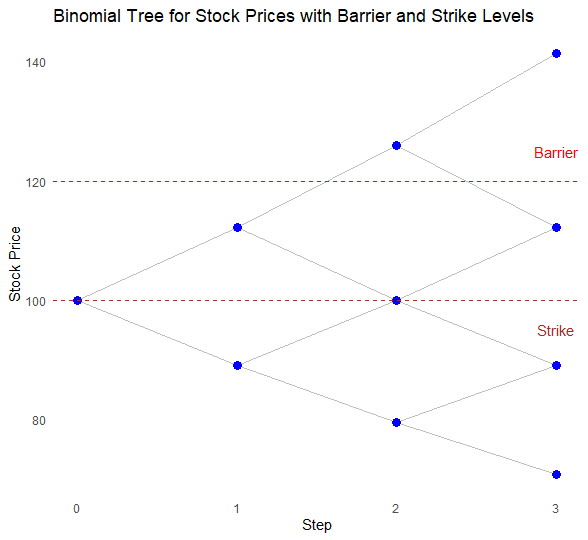
\includegraphics[width=.75\linewidth]{content/images/three-step.png}
%    \caption{Binomial Tree with Barrier Level \(B = 90\) and Strike Price \(K = 105\).}
%    \label{fig:binomial-tree}
%\end{figure}

The binomial tree method provides a flexible and intuitive framework for pricing options, including barrier options. However, as shown in this example, its computational requirements grow significantly with the number of steps \(N\), making it less efficient for path-dependent options. Alternative methods, such as Monte Carlo simulations or analytical solutions, may be more suitable for pricing complex derivatives.
